\documentclass[t, xcolor={usenames,dvipsnames,svgnames,table}]{beamer}

\usepackage[utf8]{inputenc}
\usepackage[croatian]{babel}
\usepackage{amsmath}
\usepackage{mathtools}
\usepackage{csquotes}
\usepackage{graphicx}
\graphicspath{ {images/} }

\usetheme{PaloAlto}
\usecolortheme{seahorse}

\setbeamertemplate{section page}
{
	\begin{center}
		\begin{beamercolorbox}[sep=12pt, rounded=true, center, shadow=true]{part title}
			\usebeamerfont{section title}\insertsection\par
		\end{beamercolorbox}
	\end{center}
}

\title[Karakterizacija likova]{Karakterizacija likova u dječjim pričama}
\subtitle{Diplomski rad}
\institute{Prirodoslovno matematički fakultet - Matematički odsjek}
\author[Gorana Levačić]{\textbf {Gorana Levačić \\ \footnotesize Voditelj rada: izv.~prof.~dr.~sc.~Saša Singer}}
\date{20. studenog 2016.}

\begin{document}	

\begin{frame}
	\titlepage
\end{frame}

\begin{frame}
	\tableofcontents
\end{frame}

\section{Obrada prirodnog jezika}

	\begin{frame}
		\sectionpage
	\end{frame}

	\begin{frame}
		\frametitle{\secname}
		
		Cilj diplomskog rada -- razviti sustav koji će:
		\begin{enumerate}
			\item 	prepoznati likove u dječjim pričama
			\item 	za svakog lika zaključiti je li dobar ili loš
		\end{enumerate}
		
		\medskip
		
		$\Rightarrow$ problem obrade prirodnog jezika
	
	\end{frame}
		
	\begin{frame}
		\frametitle{\secname}
		
		Objedinjuje:	
		\begin{itemize}
			\item	računarstvo
			\item 	umjetnu inteligenciju 
			\item 	računalnu lingvistiku
		\end{itemize}
		
		\medskip
		
		Problemi:
		\begin{itemize}
			\item	razumijevanje prirodnog jezika
			\item 	strojno prevođenje
			\item 	prepoznavanje govora
			\item 	generiranje teksta
		\end{itemize}
		
		\hspace{0.8em} \vdots
	
	\end{frame}
	
	\begin{frame}
		\frametitle{\secname}
		
		Problemi prepoznati u problemu karakterizacije likova:
		\begin{itemize}
			\item	prepoznavanje imenovanih entiteta
			\item	razrješavanje koreferencije
			\item 	analiza sentimenta
		\end{itemize}
	\end{frame}
	
	\begin{frame}
		\frametitle{\secname}

		Pristup rješavanju problema obrade prirodnog jezika:
		\begin{enumerate}
			\item	formalno modeliranje
			\item 	statističke metode
			\item 	strojno učenje
		\end{enumerate}
	\end{frame}


\section{Prepoznavanje imenovanih entiteta}
	
	\begin{frame}
		\sectionpage
	\end{frame}

	\begin{frame}
		\frametitle{\secname}
		
		\begin{itemize}
			\item 	prepoznavanje i klasificiranje izraza u tekstu koji se odnose na imenovane entitete
		\end{itemize}
		
		\medskip
		Imenovani entiteti:
		\begin{itemize}
			\item	osobe
			\item	lokacije
			\item 	organizacije
		\end{itemize}	
		\hspace{0.8em} \vdots
		
		\medskip
		
		\begin{displayquote}
			\textit{$\underbracket{\text{Red Riding Hood}}_{\text{Person}}$ walked through $\underbracket{\text{Grünewald}}_{\text{Location}}$ forest.}
		\end{displayquote}
		
		
	\end{frame}
	
	\begin{frame}
		\frametitle{\secname}
		
		U problemu karakterizacije likova jedna kategorija -- likovi:
		\begin{itemize}
			\item 	imenovani -- \textit{Little Red Riding Hood}
			\item	neimenovani -- \textit{evil witch}
		\end{itemize}
		
		\bigskip
		
		Postojeći NER sustavi prepoznaju samo imenovane likove
		
		$\Rightarrow$ treniranje vlastitog modela 
	
	\end{frame}
	
	\begin{frame}
		\frametitle{\secname}
		
		Metode:
		\begin{itemize}
			\item 	\textbf{skriveni Markovljevi modeli} -- pretpostavljaju da oznaka ovisi samo o toj riječi i o oznaci prethodne riječi u nizu
				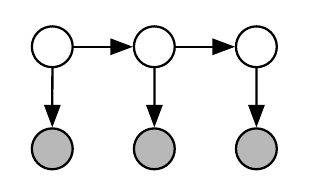
\includegraphics[scale = 0.25]{hmm.png}
			\item 	\textbf{uvjetna slučajna polja} -- za ulaz uzimaju više podataka o samoj riječi, ne promatraju nužno isključivo prethodnu oznaku \\
				\medskip
				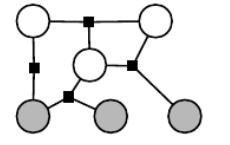
\includegraphics[scale = 0.35]{crf.png}
		\end{itemize}
		
	\end{frame}

	
\section{Razrješavanje koreferencije}
	
	\begin{frame}
		\sectionpage
	\end{frame}
	
	\begin{frame}
		\frametitle{\secname}
		
		\begin{itemize}
			\item	prepoznavanje izraza u tekstu koji se odnose na isti izvanjezični entitet
		\end{itemize}
		
		\bigskip
		
		\begin{displayquote}
			\textit{\textcolor{Blue}{She} always wore red cloak with a hood, so people called \textcolor{Blue}{her} \textcolor{BrickRed}{Little Red Riding Hood}.}
		\end{displayquote}
	\end{frame}
	
	\begin{frame}
		\frametitle{\secname}
		
		Metode:
		\begin{itemize}
			\item 	\textbf{model parova} -- promatra vjerojatnost međusobne koreferencije pojedinih parova izraza \\
					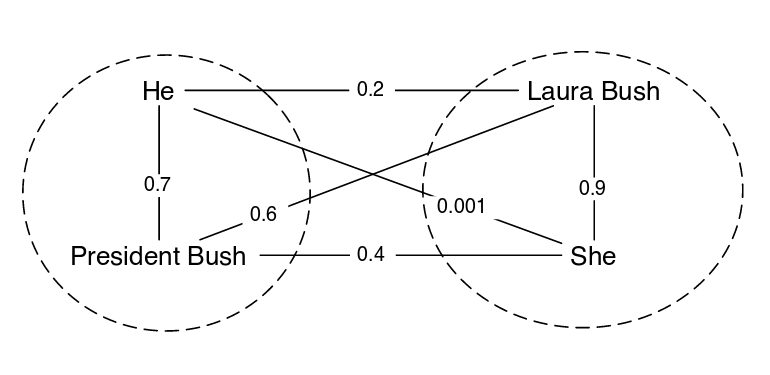
\includegraphics[scale = 0.3]{coreference_example.png}
			\item 	\textbf{model logike prvog reda} -- poopćenje prethodnog modela, prepoznaje grupe koreferentnih izraza
					
		\end{itemize}
					
	\end{frame}
	
	\begin{frame}
		\frametitle{\secname}
		
		Metode (nastavak):
		\begin{itemize}
			\item 	\textbf{metoda višeprolaznog sita} -- Stanfordov \textit{state-of-the-art} sustav \\
				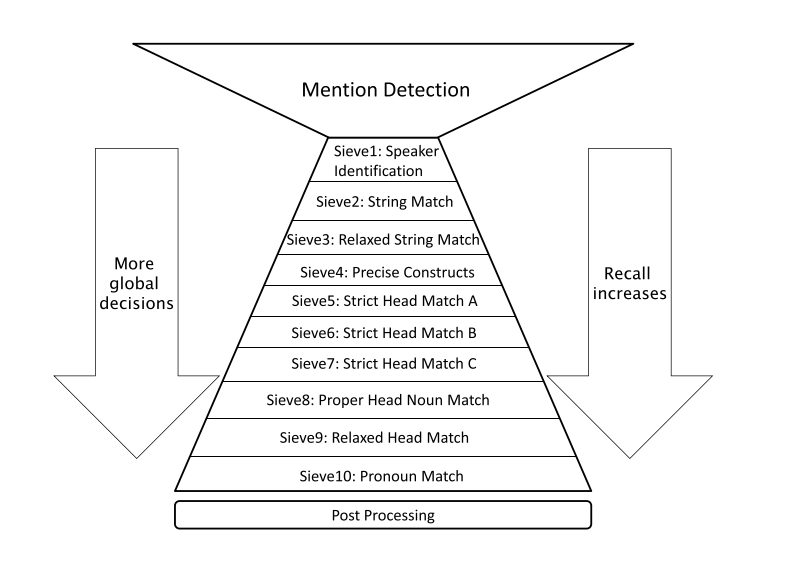
\includegraphics[scale = 0.4]{sieve.png}
			
		\end{itemize}
		
	\end{frame}


\section{Analiza sentimenta}
	
	\begin{frame}
		\sectionpage
	\end{frame}

	\begin{frame}
		\frametitle{\secname}
		
		Određivanje stava zadanog teksta:
		\begin{itemize}
			\item	pozitivan ili negativan
			\item 	subjektivan ili objektivan
			\item 	više različitih karakteristika nekog pojma
		\end{itemize}
		
		\bigskip
		
		\begin{displayquote}
			\textit{This book is not very interesting, but it has great characters.}
		\end{displayquote}
	\end{frame}
	
	\begin{frame}
		\frametitle{\secname}
		
		Metode:
		\begin{itemize}
			\item 	\textbf{"vreća riječi"} -- prikaz teksta isključivo kao skupa riječi koje ga čine
			
			\item 	\textbf{"vreća stavova"} -- promatra stavove koji se sastoje od korijena (\textit{interesting}), modifikatora (\textit{very}) i negatora (\textit{not})
			
			\item	\textbf{rekurzivni duboki modeli} -- temelje se na neuronskim mrežama, Stanfordov \textit{state-of-the-art} model \\
			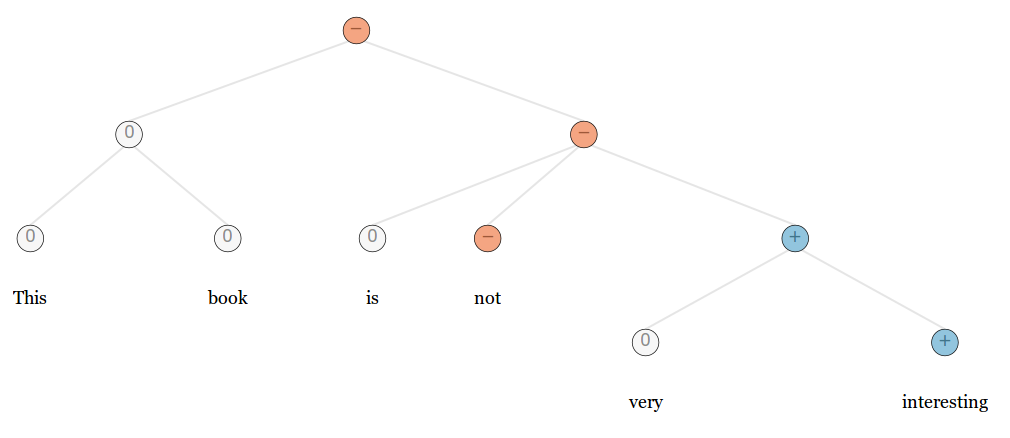
\includegraphics[scale = 0.35]{sentiment_treebank.png}
			
		\end{itemize}
		
	\end{frame}

\section{Razvoj aplikacije za karakterizaciju likova}
	
	\begin{frame}
		\sectionpage
	\end{frame}
	
	\begin{frame}
		\frametitle{\secname}
		
		Pristup:
		\begin{itemize}
			\item	programski jezik Java
			\item	upotreba \textit{Stanford CoreNLP} skupa alata za obradu prirodnog jezika
			\item 	treniranje vlastitih CRF NER modela za prepoznavanje likova
			\item 	korištenje već istreniranih modela za razrješavanje koreferencije i analizu sentimenta
		\end{itemize}
	\end{frame}
	
	\begin{frame}
		\frametitle{\secname}
		
		Testiranje:
		\begin{itemize}
			\item	Snjeguljica
			\item 	Pepeljuga
			\item 	Vuk i sedam kozlića
			\item	Pljačkaš zaručnik
		\end{itemize}
		
		\bigskip
		
		Rezultati:
		\begin{itemize}
			\item 	većinom ispravno prepoznaje likove
			\item	dobre likove koji su sretni karakterizira kao dobre
			\item 	dobre likove koji su nesretni karakterizira kao loše
			\item 	loše likove najčešće karakterizira kao loše
		\end{itemize}
		
	\end{frame}

\section{Zaključak}
	
	\begin{frame}
		\sectionpage
	\end{frame}
	
	\begin{frame}
		\frametitle{\secname}
		
		Moguća poboljšanja:
		\begin{itemize}
			\item	prepoznavanjem surečenica u rečenici
			\item 	promatranjem samo onih rečenica u kojima je subjekt lik
			\item 	treniranjem zasebnog modela za analizu sentimenta
		\end{itemize}
		
		\bigskip
		
		Drugi pristup rješavanju problema:
		\begin{itemize}
			\item	treniranjem jedinstvenog modela nad označenim podacima
			\item	oznake \textit{lik, karakter} za pojedine dijelove teksta
			\item 	neuronske mreže
		\end{itemize}
		
	\end{frame}


\section{Zaključak}



\end{document}